\documentclass[titlepage,UTF8,zihao=-4]{ctexart}

\usepackage{tikz}

\usepackage{amssymb}
\usepackage{amsmath}
\usepackage{array}

\usepackage{graphicx}

\usepackage[a4paper,left=2cm,right=2cm,top=2.5cm,bottom=2.5cm]{geometry}

\usepackage{fancyhdr}
\pagestyle{fancy}
\fancyhead[L,C,R]{}  \fancyfoot[C]{\thepage} \fancyfoot[L,R]{} \renewcommand{\headrulewidth}{0.0cm}
\renewcommand{\footrulewidth}{0.0cm}

\usepackage{hyperref}
\usepackage{float}
\usepackage{ulem}


\usepackage{tabularx}
\usepackage{booktabs}







\title{用神经网络识别手写字体\\以MNIST数据集为例}
\author{Yaohui Li}
\date{\today}

\begin{document}

\maketitle
\section{写在前面}
本教程的愿景是从问题出发,教会读者实现机器学习领域中深度学习方向的"Hello,world!"项目——运用神经网络识别手写字体(以MNIST数据集为例)。本教程是注重实践的教程,不涉及对理论知识的过多讨论。

教程假设读者具备以下基础:
\begin{itemize}
    \item 一些高等数学的基础知识
    \item 了解深度学习的一些基本理论
    \item 少量C++程序设计的知识
\end{itemize}

读者如果对深度学习的基本理论没有任何了解,可以参考文献\cite{LH,MN},C++程序设计的基本知识则可以参考文献\cite{CPP}。实际上,读者只要懂得如何编译、链接程序,就可以顺利运行本教程附带的程序,本教程附带的程序已上传至\url{https://github.com/Yaohui1996/ASimpleNNCMake}。

阅读完本教程,读者应该就有能力实现自己的神经网络并用它识别MNIST数据集中的手写字体(实际上,本教程附带的程序是一个简单的神经网络框架,该框架可以任意指定网络层数和每一层的神经元个数)。

\textbf{本教程适合}:了解一些简单的深度学习知识,希望能抛开使用现有的框架(Tensorflow、PyTorch等),自己动手实现自己的神经网络的读者。

\textbf{本教程不适合}:完全不了解深度学习或完全没有程序设计经验的读者。



\section{本教程构建的程序所要解决的问题}
当我们看到由(\hyperref[im1]{图1})中$28\times28$个像素点构成的图像时,会很自然地想到这张图像想要表达的含义是阿拉伯数字“5”,但是,计算机却没有那么聪明,怎么才能让计算机认出这张图是"5",并且让计算机看到类似的其它图像(\hyperref[im2]{图2}),都能认出这是"5"。甚至,当计算机看到其它图像(\hyperref[im3]{图3})的时候,也能认出相应的数字\footnote{5 0 4 1 9 2 1 3},这便是我们要做的工作。

本教程以MNIST数据集为例子,想要深入了解MNIST数据集,可以登录\url{http://yann.lecun.com/exdb/mnist/}查看相关介绍,这里不对该数据集做过多的介绍。

\begin{figure}[htbp] 
    \centering   
    
\includegraphics[width=8 cm]{./Images/0.png}
    \caption{MNIST训练集中的第一张图像}\label{im1}
\end{figure}

\begin{figure}[htbp]
    \centering
    
\includegraphics[width=4 cm]{./Images/35.png}
    
\includegraphics[width=4 cm]{./Images/47.png}
    
\includegraphics[width=4 cm]{./Images/65.png}
    
\includegraphics[width=4 cm]{./Images/100.png}
    \\[2 pt]
    
\includegraphics[width=4 cm]{./Images/138.png}
    
\includegraphics[width=4 cm]{./Images/145.png}
    
\includegraphics[width=4 cm]{./Images/173.png}
    
\includegraphics[width=4 cm]{./Images/175.png}
    \caption{MNIST训练集中其它的“5”}\label{im2}
\end{figure}

\begin{figure}[htbp]
    \centering
    
\includegraphics[width=4 cm]{./Images/0.png}
    
\includegraphics[width=4 cm]{./Images/1.png}
    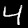
\includegraphics[width=4 cm]{./Images/2.png}
    
\includegraphics[width=4 cm]{./Images/3.png}
    \\[2 pt]
    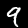
\includegraphics[width=4 cm]{./Images/4.png}
    
\includegraphics[width=4 cm]{./Images/5.png}
    
\includegraphics[width=4 cm]{./Images/6.png}
    
\includegraphics[width=4 cm]{./Images/7.png}
    \caption{MNIST训练集中其它的图像}\label{im3}
\end{figure}

当然,计算机无法直接读取一张图像,计算机更擅长处理数字,我们首先需要将图像转换成数字。

由于MNIST数据集中所有的图像都是由$28\times28$个像素点组成的黑白图片(灰度图)\footnote{实际上,该数据集是以二进制文件存储的,这里的图像是解码后的结果},每个像素点蕴含一个灰度信息,取值是$[0,255]$中的整数,其中0代表最暗(全黑),255代表最亮(全白)。那么,每一张图像都有一个$28\times28$的矩阵与之对应。更一般地,不如将矩阵拉直,转换成一个向量$x\in \mathbb{R}^{n}$,其中$n=28 \times 28=784$。

我们的目标是编写这样一个程序,姑且称之为程序$P$,我们希望将向量$x$输入程序$P$,经过计算后,得到的计算结果能够与向量$x$对应的图像所对应的数字一一对应。这样便能在任意输入一张图像的情况下,根据$P$的计算结果,知道这张图像代表哪一个阿拉伯数字。

现在需要知道的一个事实是:程序$P$的结构类似于(\hyperref[im4]{图4}),输入层的$n$个神经元代表向量$x$的$n$个分量,输出层的10个神经元分别代表数字0-9。我们希望在给定一个向量$x$的情况下(比如在$x$对应的图像显示的数字为5时),输出层对应的神经元的值最大(神经元5的数值最大(从0开始计数))。

我们面临的问题就这样描述完毕了,更多的细节将在后文讨论,如果读者对所面临的问题还存在疑惑,不妨重复阅读这一节的内容。

\begin{figure}[htpb]
    \centering
    \begin{tikzpicture}[every node/.style={align=center}]
        \foreach \i in {5,6,...,10}{\coordinate (one\i) at (0,\i); }
        \foreach \i in {1,2,...,16}{\coordinate (two\i) at (4,\i); }
        \foreach \i in {1,2,...,16}{\coordinate (three\i) at (8,\i); }
        \foreach \i in {3,4,...,12}{\coordinate (four\i) at (12,\i); }
        
        \foreach \i in {5,6,...,10} {\draw(one\i) circle [radius=0.2 cm];}
        \foreach \i in {1,2,...,16} {\draw (two\i) circle [radius=0.2 cm]; }
        \foreach \i in {1,2,...,16} {\draw (three\i) circle [radius=0.2 cm]; }
        \foreach \i in {3,4,...,12} {\draw (four\i) circle [radius=0.2 cm]; }
        
        \foreach \i in {5,6,...,10}{ \foreach \j in {1,2,...,16} { \draw[ultra thin] (one\i) -- (two\j); }  }
        \foreach \i in {1,2,...,16}{ \foreach \j in {1,2,...,16} { \draw[ultra thin] (two\i) -- (three\j); }  }
        \foreach \i in {1,2,...,16}{ \foreach \j in {3,4,...,12} { \draw[ultra thin] (three\i) -- (four\j); }  }
        
        \node[above of = two16, node distance=1cm] (hl) {隐藏层1};
        \node[left of=hl,node distance=4cm] {输入层};
        \node[right of=hl,node distance=4cm] (h2){隐藏层2};
        \node[right of=h2,node distance=4cm] (h3){输出层};
        
        \node[left of=one5,node distance=2cm](l5){$x_{n}$};
        \node[left of=one6,node distance=2cm](l6){$x_{n-1}$};
        \node[left of=one7,node distance=2cm](l7){$\vdots$};
        \node[left of=one8,node distance=2cm](l8){$\vdots$};
        \node[left of=one9,node distance=2cm](l9){$x_{2}$};
        \node[left of=one10,node distance=2cm](l10){$x_{1}$}; 
        
        \node[right of=four3,node distance=2cm]{$9$};
        \node[right of=four4,node distance=2cm]{$8$};
        \node[right of=four5,node distance=2cm]{$7$};
        \node[right of=four6,node distance=2cm]{$6$};
        \node[right of=four7,node distance=2cm]{$5$};
        \node[right of=four8,node distance=2cm]{$4$};
        \node[right of=four9,node distance=2cm]{$3$};
        \node[right of=four10,node distance=2cm]{$2$};
        \node[right of=four11,node distance=2cm]{$1$};
        \node[right of=four12,node distance=2cm]{$0$};
        
    \end{tikzpicture}
    \caption{神经网络示意图}\label{im4}
\end{figure}

\section{神经网络模型是如何工作的}
实际上,本教程所使用的模型是一个多层感知机模型,这是深度学习的一个基本模型。有关感知机模型的更多内容,可以参考文献\cite{LH,MN}。本教程着眼于实践,对于理论部分不会大篇幅介绍,只给出一些需要用到的事实。

为了描述多层感知机模型是如何工作的,不得不定义一些必要的符号(实际上这些奇怪的数学符号一眼看上去就很令人头大),如果一次性把所有需要用到的符号列出来,难免会造成阅读上的负担,所以,本教程采用一种“过程式”的方法行文,用例子进行讲解,只在必要的时候定义符号。

假设我们所使用的神经网络正是(\hyperref[im4]{图4})所示的神经网络,这个神经网络一共有4层,第一层为输入层(有784个神经元),第二层和第三层为隐藏层(分别有16个神经元),第四层为输出层(有10个神经元)。

以MNIST训练集中第一章图像为例(\hyperref[im1]{图1}),其图像对应的$28\times28$的矩阵如(\hyperref[matrix]{图5})所示\footnote{拉伸成向量的话不便于展示,这里就展示矩阵}。细心的读者可能会发现,矩阵的形状好像一个数字“5”。

\begin{figure}
    \begin{equation*}
    \begin{bmatrix}
    \addtocounter{MaxMatrixCols}{28}
    \begin{smallmatrix}
    0& 0& 0& 0& 0& 0& 0& 0& 0& 0& 0& 0& 0& 0& 0& 0& 0& 0& 0& 0& 0& 0& 0& 0& 0& 0& 0& 0 \\
    0& 0& 0& 0& 0& 0& 0& 0& 0& 0& 0& 0& 0& 0& 0& 0& 0& 0& 0& 0& 0& 0& 0& 0& 0& 0& 0& 0 \\
    0& 0& 0& 0& 0& 0& 0& 0& 0& 0& 0& 0& 0& 0& 0& 0& 0& 0& 0& 0& 0& 0& 0& 0& 0& 0& 0& 0 \\
    0& 0& 0& 0& 0& 0& 0& 0& 0& 0& 0& 0& 0& 0& 0& 0& 0& 0& 0& 0& 0& 0& 0& 0& 0& 0& 0& 0 \\
    0& 0& 0& 0& 0& 0& 0& 0& 0& 0& 0& 0& 0& 0& 0& 0& 0& 0& 0& 0& 0& 0& 0& 0& 0& 0& 0& 0 \\
    0& 0& 0& 0& 0& 0& 0& 0& 0& 0& 0& 0& 3& 18& 18& 18& 126& 136& 175& 26& 166& 255& 247& 127& 0& 0& 0& 0 \\
    0& 0& 0& 0& 0& 0& 0& 0& 30& 36& 94& 154& 170& 253& 253& 253& 253& 253& 225& 172& 253& 242& 195& 64& 0& 0& 0& 0 \\
    0& 0& 0& 0& 0& 0& 0& 49& 238& 253& 253& 253& 253& 253& 253& 253& 253& 251& 93& 82& 82& 56& 39& 0& 0& 0& 0& 0 \\
    0& 0& 0& 0& 0& 0& 0& 18& 219& 253& 253& 253& 253& 253& 198& 182& 247& 241& 0& 0& 0& 0& 0& 0& 0& 0& 0& 0 \\
    0& 0& 0& 0& 0& 0& 0& 0& 80& 156& 107& 253& 253& 205& 11& 0& 43& 154& 0& 0& 0& 0& 0& 0& 0& 0& 0& 0 \\
    0& 0& 0& 0& 0& 0& 0& 0& 0& 14& 1& 154& 253& 90& 0& 0& 0& 0& 0& 0& 0& 0& 0& 0& 0& 0& 0& 0 \\
    0& 0& 0& 0& 0& 0& 0& 0& 0& 0& 0& 139& 253& 190& 2& 0& 0& 0& 0& 0& 0& 0& 0& 0& 0& 0& 0& 0 \\
    0& 0& 0& 0& 0& 0& 0& 0& 0& 0& 0& 11& 190& 253& 70& 0& 0& 0& 0& 0& 0& 0& 0& 0& 0& 0& 0& 0 \\
    0& 0& 0& 0& 0& 0& 0& 0& 0& 0& 0& 0& 35& 241& 225& 160& 108& 1& 0& 0& 0& 0& 0& 0& 0& 0& 0& 0 \\
    0& 0& 0& 0& 0& 0& 0& 0& 0& 0& 0& 0& 0& 81& 240& 253& 253& 119& 25& 0& 0& 0& 0& 0& 0& 0& 0& 0 \\
    0& 0& 0& 0& 0& 0& 0& 0& 0& 0& 0& 0& 0& 0& 45& 186& 253& 253& 150& 27& 0& 0& 0& 0& 0& 0& 0& 0 \\
    0& 0& 0& 0& 0& 0& 0& 0& 0& 0& 0& 0& 0& 0& 0& 16& 93& 252& 253& 187& 0& 0& 0& 0& 0& 0& 0& 0 \\
    0& 0& 0& 0& 0& 0& 0& 0& 0& 0& 0& 0& 0& 0& 0& 0& 0& 249& 253& 249& 64& 0& 0& 0& 0& 0& 0& 0 \\
    0& 0& 0& 0& 0& 0& 0& 0& 0& 0& 0& 0& 0& 0& 46& 130& 183& 253& 253& 207& 2& 0& 0& 0& 0& 0& 0& 0 \\
    0& 0& 0& 0& 0& 0& 0& 0& 0& 0& 0& 0& 39& 148& 229& 253& 253& 253& 250& 182& 0& 0& 0& 0& 0& 0& 0& 0 \\
    0& 0& 0& 0& 0& 0& 0& 0& 0& 0& 24& 114& 221& 253& 253& 253& 253& 201& 78& 0& 0& 0& 0& 0& 0& 0& 0& 0 \\
    0& 0& 0& 0& 0& 0& 0& 0& 23& 66& 213& 253& 253& 253& 253& 198& 81& 2& 0& 0& 0& 0& 0& 0& 0& 0& 0& 0 \\
    0& 0& 0& 0& 0& 0& 18& 171& 219& 253& 253& 253& 253& 195& 80& 9& 0& 0& 0& 0& 0& 0& 0& 0& 0& 0& 0& 0 \\
    0& 0& 0& 0& 55& 172& 226& 253& 253& 253& 253& 244& 133& 11& 0& 0& 0& 0& 0& 0& 0& 0& 0& 0& 0& 0& 0& 0 \\
    0& 0& 0& 0& 136& 253& 253& 253& 212& 135& 132& 16& 0& 0& 0& 0& 0& 0& 0& 0& 0& 0& 0& 0& 0& 0& 0& 0 \\
    0& 0& 0& 0& 0& 0& 0& 0& 0& 0& 0& 0& 0& 0& 0& 0& 0& 0& 0& 0& 0& 0& 0& 0& 0& 0& 0& 0 \\
    0& 0& 0& 0& 0& 0& 0& 0& 0& 0& 0& 0& 0& 0& 0& 0& 0& 0& 0& 0& 0& 0& 0& 0& 0& 0& 0& 0 \\
    0& 0& 0& 0& 0& 0& 0& 0& 0& 0& 0& 0& 0& 0& 0& 0& 0& 0& 0& 0& 0& 0& 0& 0& 0& 0& 0& 0 \\
    \end{smallmatrix}
    \end{bmatrix}
    \end{equation*}
    \caption{\hyperref[im1]{图1}所示的图像对应的矩阵}\label{matrix}
\end{figure}

把这个矩阵的第2行拼接到第1行后面,第3行拼接到原始矩阵的第2行,以此类推,拉直成为一个行向量,姑且称其转置后的列向量为$x$,$x\in \mathbb{R}^{784}$。

接下来我们就要开始计算啦!(事实上,这个过程一般被成为前向传播,如果读者实在好奇有关前向传播的理论知识,可以查阅文献\cite{MN,QXP})

为了把计算流程说清楚,不得不引入一些符号:

用符号$l$表示第$l$层,用符号$L$表示最后一层,输入层$l=0$。本例中$l=\{0,1,2,3\}$,$L=3$。

用符号$a^l_j$表示第$l$层的第$j$个神经元的激活值,$a^l$表示第$l$层所有神经元激活值组成的向量。

用符号$w_{kj}^l$表示第$l-1$层第$j$个神经元与第$l$层第$k$个神经元连线的权重,这些权重构成矩阵$w^l$,表示从第$l-1$层到第$l$层的权重矩阵。

用符号$b^l_j$表示第$l$层的第$j$个神经元的bias,$b^l$表示第$l$层所有神经元bias组成的向量。

\textbf{第一步。} 将$x$输入网络,即令$a^0=x$。

\textbf{第二步。} 随机初始化$w^l$和$b^l$。(本例中$l=\{0,1,2,3\}$)

\textbf{第三步。} 交替计算$z^l$、$a^l$,计算方法为:(本例中$l=\{0,1,2,3\}$)

\begin{equation*}
    z^l = w^la^{l-1}+b^l 
\end{equation*}

\begin{equation*}
    a^l = f(z^l) 
\end{equation*}

其中\footnote{该函数一般被称为sigmoid函数}:
\begin{equation*}
f(x) = \frac{1}{1+e^{-x}}
\end{equation*}

\textbf{第四步。} 通过输出向量$a^L$获得识别的结果。

对于本例,经过上述运算\footnote{主要是一系列的线性变换,读者可以回忆一下线性代数的知识},一定可以得到维数为10的向量$a^L$。

我们\textbf{期望的输出}为:
\begin{equation*}
y^T=
\begin{bmatrix}
\addtocounter{MaxMatrixCols}{28}
0.00 &
0.00 &
0.00 &
0.00 &
0.00 &
1.00 &
0.00 &
0.00 &   
0.00 &
0.00 
\end{bmatrix}
\end{equation*}

也就是希望输出向量的第6个分量尽可能接近1,其它分量尽可能接近0。

\textbf{实际上},${a^{L}}^T$可能为:
\begin{equation*}
    \begin{bmatrix}
    \addtocounter{MaxMatrixCols}{28}
    0.31 &
    0.02 &
    0.12 &
    0.44 &
    0.79 &
    0.97 &
    0.21 &
    0.53 &   
     0.22 &
    0.67 
    \end{bmatrix}
\end{equation*}

该向量第6个分量的值最大,就认为输入向量$x$代表的图像为数字5的\textbf{可能性}更大。

如果${a^{L}}^T$为:
\begin{equation*}
\begin{bmatrix}
\addtocounter{MaxMatrixCols}{28}
0.31 &
0.02 &
0.12 &
0.44 &
0.79 &
0.07 &
0.21 &
0.53 &   
0.22 &
0.67 
\end{bmatrix}
\end{equation*}

就认为输入向量$x$代表的图像为数字4的\textbf{可能性}更大。,但实际上该图像为数字5,说明识别误差较大,需要提高准确度。

不管怎样,对于输入向量$x$而言,我们期望的${a^{L}}^T$始终为:
\begin{equation*}
\begin{bmatrix}
\addtocounter{MaxMatrixCols}{28}
0.00 &
0.00 &
0.00 &
0.00 &
0.00 &
1.00 &
0.00 &
0.00 &   
0.00 &
0.00 
\end{bmatrix}
\end{equation*}

阅读到这里,读者或许可以意识到,决定识别准确的因素有输入向量$x$,权重矩阵$w$,bias向量$b$\footnote{后文用$w$和$b$分别表示所有的$w^{l}_{jk}$和$b^{l}_{j}$构成的集合}。在给定图像的情况下,$x$是一个常量。对于一个输入样本而言,如果可以找到“最好的”$w$和$b$,使输出向量达到或尽可能接近我们的期望,这个神经网络就能有不错的表现。

\section{如何找到最好的$w$和$b$}

假设期望输出为$y$,实际输出为${a^{L}}^T$,如果定义\footnote{误差函数可以有多种定义方式,这里定义成二次函数的一个原因是导函数很容易计算}:
\begin{equation*}
    C =  {\Vert a^L - y \Vert}^2
\end{equation*}

为误差,那么当且仅当$a^L = y$时,误差为0,即使无法达到这样的条件,我们也希望能使误差尽可能地小。此时对应的$w$和$b$就是“最好的”。

上述讨论基于一个输入样本,对于多个输入样本,使$C$的平均值最小的$w$和$b$就是“最好的”。如何找到“最好的”$w$和$b$?这是一个非常难的问题。

找到“最好的”$w$和$b$是一个目标函数连续的无约束优化问题,由微积分的相关知识可知,最优解在驻点处产生\footnote{实际上,该问题一般非凸,找到的最优解是局部最优解}。此外,在某点处,沿该处的梯度方向移动一个很小的步长,函数值上升最快。为了取得比当前的$C$更小的$C$,可以沿梯度的反方向移动。问题变为了如何求梯度?

读者或许能够意识到,该网络存在以下的函数关系:
\begin{align*}
z^l &= g(a^{l-1},w^l,b^l) \\
a^l &= f(z^{l}) \\
C &= h(a^L) 
\end{align*}

那么\footnote{这里只举了2个例子,分别为$\frac{\partial C}{\partial w^L}$和$\frac{\partial C}{\partial b^{L}}$}:
\begin{align*}
\frac{\partial C}{\partial w^{L}} &= \frac{\partial z^L}{\partial w^{L}}\frac{\partial a^L}{\partial z^L}\frac{\partial C}{\partial a^L} \\
&= 2a^{L-1} f^{'}(z^L)(a^L-y) \\
\frac{\partial C}{\partial b^{L}} &= \frac{\partial z^L}{\partial b^{L}}\frac{\partial a^L}{\partial z^L}\frac{\partial C}{\partial a^L} \\
&= 2 f^{'}(z^L)(a^L-y) 
\end{align*}

类似地可以计算其它层的偏导数。

这里给出计算梯度的反向传播(Back Propagation)算法,反向传播算法正是链式法则(Clain Rule)的应用结果,其证明过程可参考文献\cite{MN,QXP}。

在开始介绍反向传播的计算流程之前,首先定义第$l$层第$j$个神经元的$\delta_j^l=\frac{\partial C}{\partial z_j^l}$,这些单元共同构成向量$\delta^l$。

在前向传播的基础上:

\textbf{第五步。} 计算$\delta^L = \frac{\partial C}{\partial a^L} \odot f^{'}(z^L)$。\footnote{$s \odot t = u$的含义为:$s_jt_j =u_j $}

\textbf{第六步。} 对于$l = \{L-1,L-2,\dots,2\}$,计算$\delta^l = (w^{l+1})^T\delta^{l+1} \odot f^{'}(z^L) $。

\textbf{第七步。} 计算梯度$\frac{\partial C}{\partial b^l} = \delta^l$,$\frac{\partial C}{\partial w^l} = \delta^l(a^{l-1})^T  $。

在搞明白符号含义的前提下,\textbf{第一步}到\textbf{第七步},就是一个完整的计算流程。需要注意的是,上述例子仅仅使用了一个样本,实际情况的样本数目更多。对于多个样本而言,可以在每次输入样本后计算梯度并更新$w$和$b$(随机梯度下降 Stochastic Gradient Descent),也可以将所有样本的梯度计算出来取平均值,进行一次更新(梯度下降 Gradient Descent)。此外,对于随机梯度下降,还可以预先把训练集划分为多个子集(batch),每次输入一个batch的样本计算梯度并求平均值更新$w$和$b$。本教程采用随机梯度下降的优化方法,且每输入一个样本都更新一次$w$和$b$。

\section{程序实现}
本教程附带的程序已上传至\url{https://github.com/Yaohui1996/ASimpleNNCMake},感兴趣的读者可以下载下来编译运行。

首先将项目文件克隆到本地,使用“cd”命令进入“build”文件夹(\hyperref[step1]{图6})。使用命令“./ASimpleNNCMake”运行程序(\hyperref[step2]{图7})。

\begin{figure}[H] 
    \centering   
    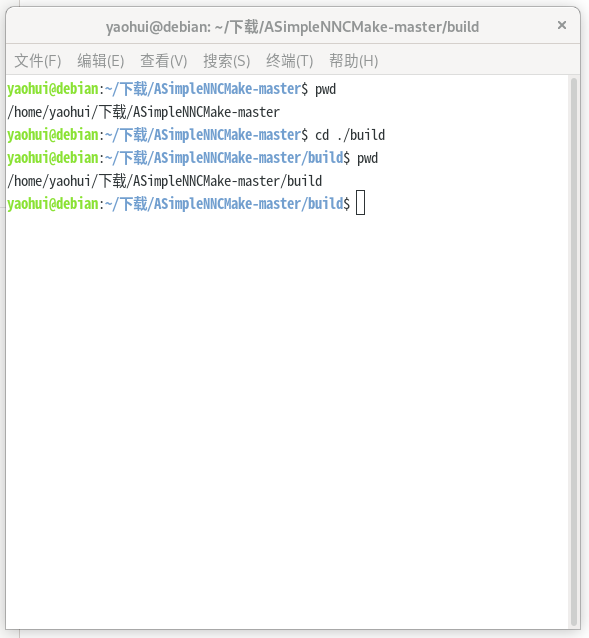
\includegraphics[width=16 cm]{./Images/step1.png}
    \caption{进入build文件夹}\label{step1}
\end{figure}

\begin{figure}[H] 
    \centering   
    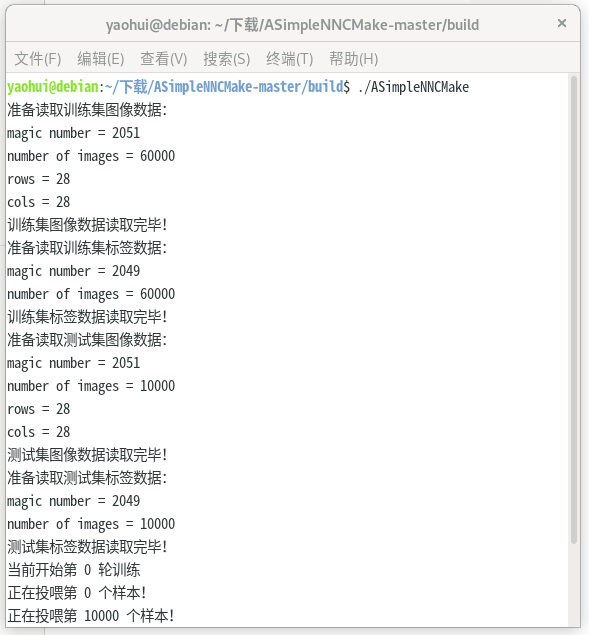
\includegraphics[width=16 cm]{./Images/step2.png}
    \caption{运行程序}\label{step2}
\end{figure}

该实现不是最快的实现,代码也不是最优美的,仅供读者参考。

\begin{thebibliography}{99}
    \bibitem{LH} 李航 <统计学习方法 2th> 
    \bibitem{MN} Michael Nielsen <Neural Networks and Deep Learning> 
    \bibitem{QXP} 邱锡鹏 <神经网络与深度学习>  \url{https://github.com/nndl/nndl.github.io}
    \bibitem{CPP} Stanley B. Lippman / Josée Lajoie / Barbara E. Moo <C++ Primer 5th> 
    
\end{thebibliography}


\end{document}